\section{Initially Random, Greedy Deployment}
\label{sec:initially_random_greedy}

Combining the random and greedy deployment schemes allows us to inject some of
the uncertainty around which reactor will be deployed at any given time while
ensuring that the demand is met in a reasonably computationally efficient
manner. This scheme does not give us more insight than the random or greedy
deployment schemes it merely allows us to leverage the strengths of both.

In this deployment scheme, we randomly deploy reactors until a reactor bigger
than the remaining capacity is proposed for each year, then fill the remaining
capacity with a greedy algorithm. We outline this scheme in Figure
\ref{fig:init_random_greedy_diagram}, which shows the two loops (first random,
then greedy) in the logic from the top down.

\begin{figure}[H]
    \centering
    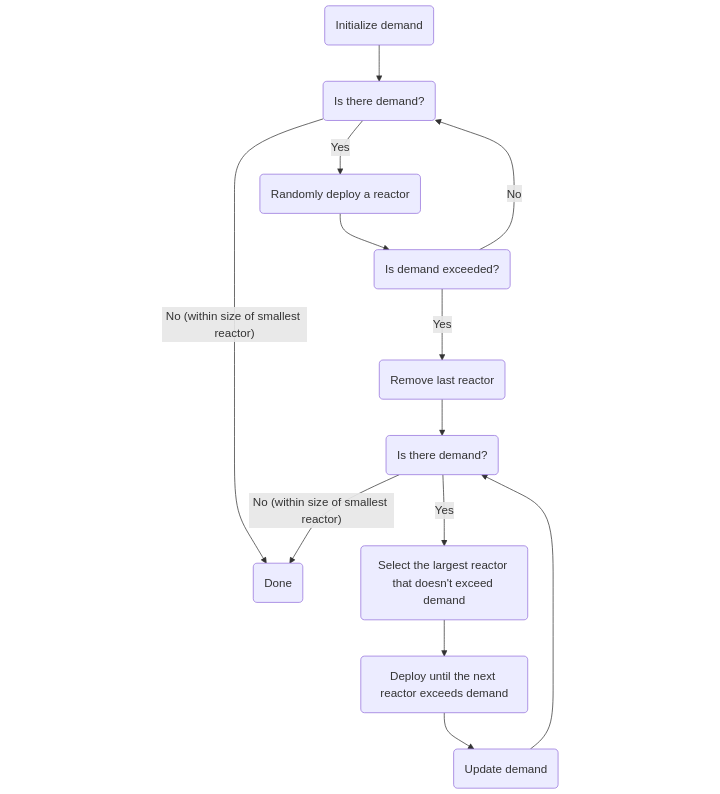
\includegraphics[scale=0.7]{images/schemes/random_greedy_diagram.png}
    \caption{Initially Random, Greedy Deployment Diagram}
    \label{fig:init_random_greedy_diagram}
\end{figure}

As highlighted in Section \ref{sec:random_deployment}, we did not implement the
initially random, greedy deployment scheme to capture additional realism in the
deployment problem. This scheme combines random and greedy deployment schemes
and inherits their realistic and unrealistic elements. The random deployment
scheme captures some of the complexity of the deployment problem but does not
guarantee the capture of the nuance of future user needs. The greedy deployment
scheme captures the efficiency of the deployment problem but does not capture
the complexity of the deployment problem. This scheme is a compromise between
the two and does not capture the nuance of the deployment problem.

The degree to which this scheme captures features of the random or greedy
deployment schemes varies with the number of reactors deployed in the random
phase. Instead of randomly deploying until the demand is met, this
implementation randomly deploys until the selected reactor exceeds the demand.
This means that when the reactors are different sizes, there is a chance that
the random phase will deploy a reactor that is much larger than the demand, and
the greedy phase will make up more of the deployment.


(((((((((The seed is set to 20240527121205)))))))))


\subsection{Number of Reactors}

% describe the difference between BAU and D2 in terms of metric

% Show total number of reactors multi fuel
\begin{figure}[H]
    \subfloat[No Growth \label{fig:rand_greed_mf_ng_reactors}]{%
      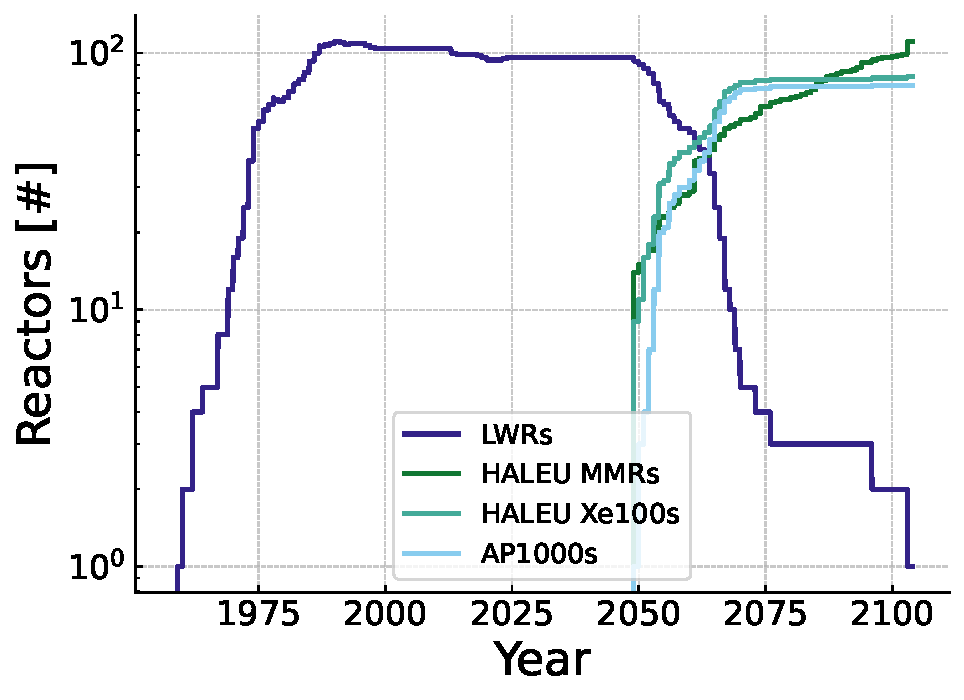
\includegraphics[width=0.495\textwidth]{images/results/multi_drgng_reactors.pdf}
   }
    \hfill
    \subfloat[Double \label{fig:rand_greed_mf_d2_reactors}]{%
      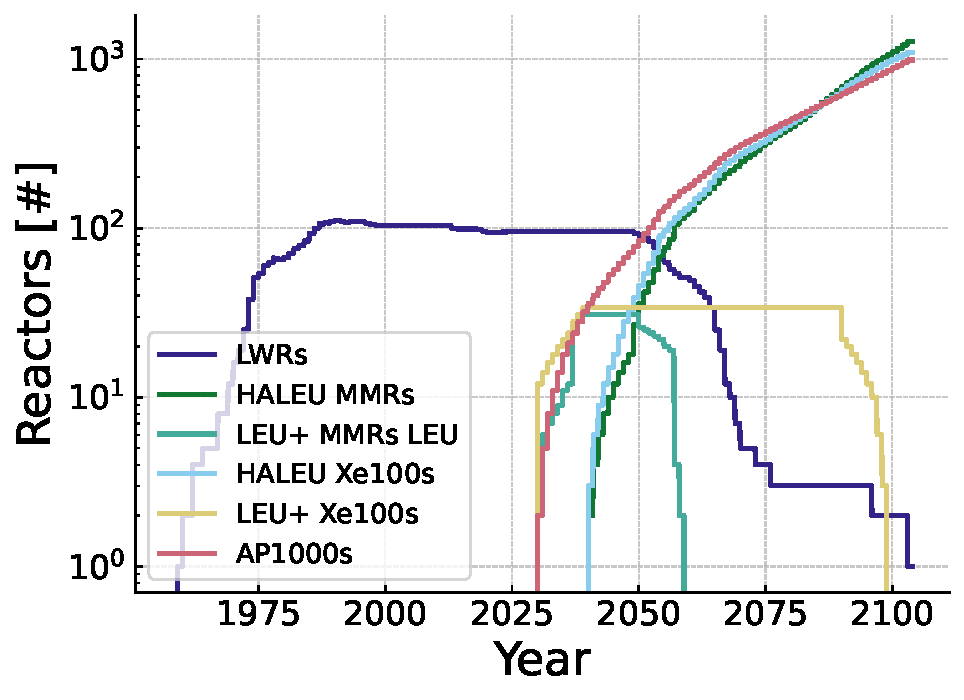
\includegraphics[width=0.495\textwidth]{images/results/multi_drg2_reactors.pdf}
   }
    \caption{Multi fuel initially random, then greedy reactor deployment.}
    \label{fig:rand_greed_mf_reactors}
  \end{figure}

% talk about the rate of deployment

% talk about the context of expanding energy needs

% talk about the workers

\begin{figure}[H]
    \subfloat[No Growth \label{fig:rand_greed_of_ng_reactors}]{%
      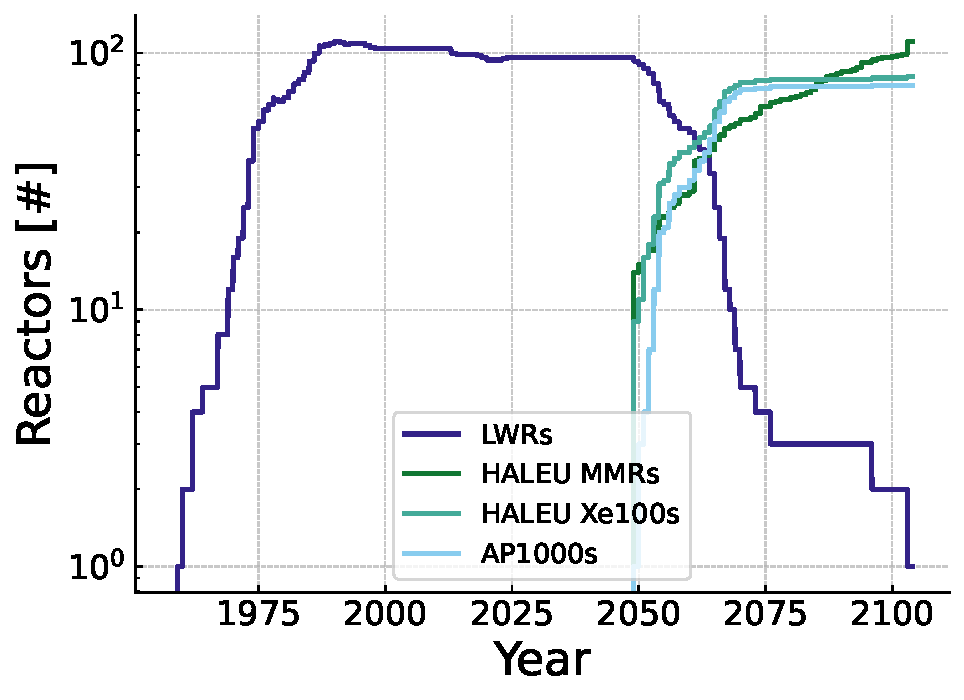
\includegraphics[width=0.495\textwidth]{images/results/one_drgng_reactors.pdf}
   }
    \hfill
    \subfloat[Double \label{fig:rand_greed_of_d2_reactors}]{%
      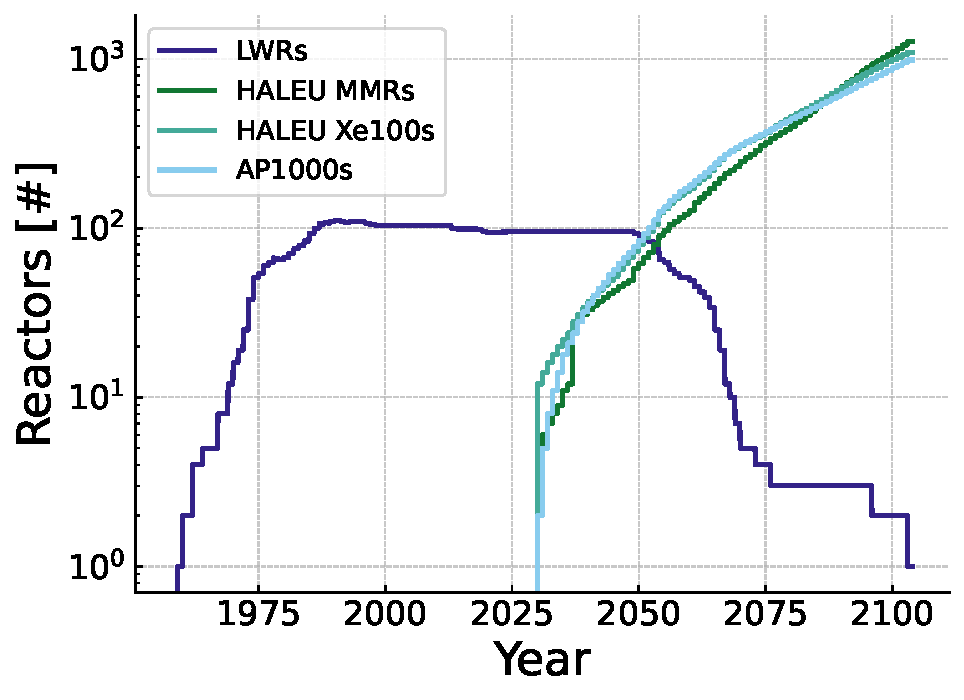
\includegraphics[width=0.495\textwidth]{images/results/one_drg2_reactors.pdf}
   }
    \caption{Single fuel initially random, then greedy reactor deployment.}
    \label{fig:rand_greed_of_reactors}
  \end{figure}

\subsection{SWU Results}

% talk about the types of category facility

% talk about the SWU capacity

% show the total SWU capacity

% talk about international trade


\subsection{Fresh Fuel Results}

% talk about the types of fuel

% show total fresh fuel

% talk about transportation of fuel


\subsection{Used Fuel Results}

% show total used fuel

% talk about repositories